%
% Contains information about the site, such as directions, how to check-in, check-out, parking
% what services are available ... and not.  Stuff like that.
%

\chapter{Pre-Flight Procedures}

\section*{Find Us Online}

You can find us online at \url{https://www.tothemoonburn.com/}.  We also have a Facebook page at \href{https://www.facebook.com/groups/1686191044986642/?ref=bookmarks}{``To The Moon - An East TN River Burn''}.

\section*{Landing Site}

\begin{figure}[!h]
\centering
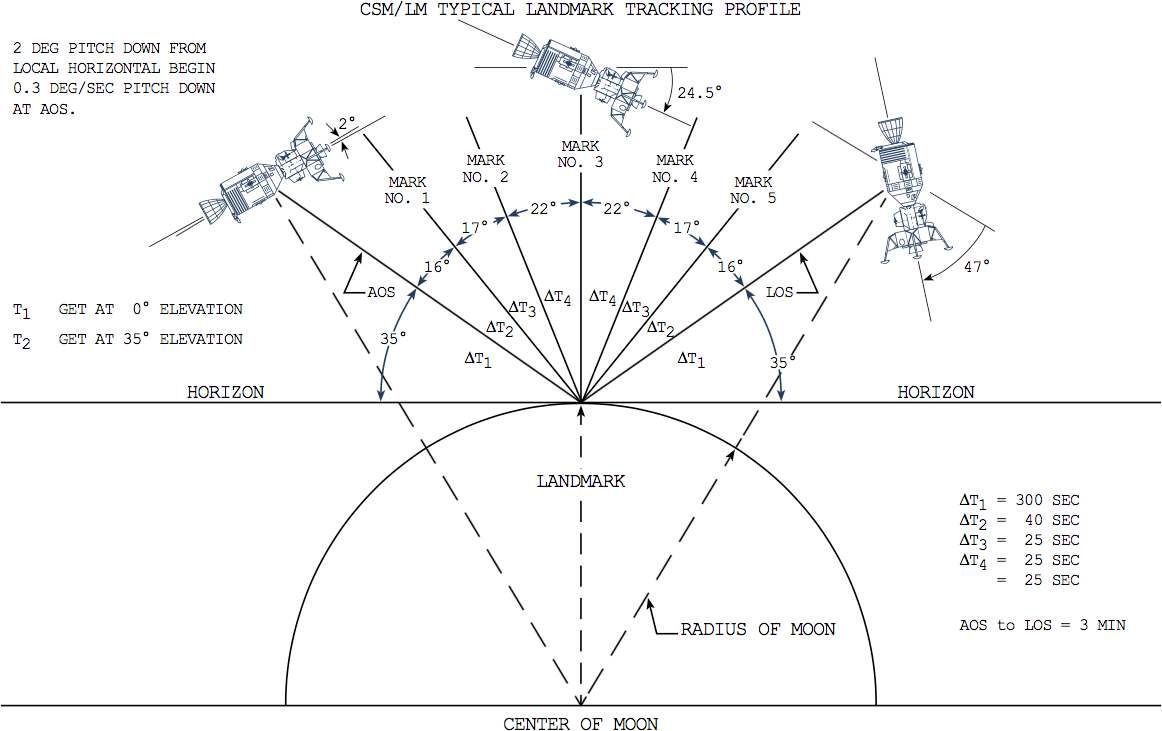
\includegraphics[width=0.9\textwidth]{images/landmarktracking.png}
% \caption{}
\label{image:landmarktracking}
\end{figure}

\begin{multicols}{3}

\subsection*{Landing Coordinates}
% \begin{quote}
36\si{\degree}31'59.0"N 83\si{\degree}08'57.0"W\\
\href{https://goo.gl/maps/pc3gYuNiF2r}{36.533051, -83.149169}
% \end{quote}

\subsection*{Address}
% \begin{quote}
Spirit Crossing\\
343 Clinch River Circle\\
Sneedville, Tennessee
% \end{quote}

\subsection*{Nearest Hospital}
% \begin{quote}
Hancock County Hospital\\
1519 Main St,\\
Sneedville, TN 37869
% \end{quote}

\end{multicols}

\begin{sidewaysfigure}[H]
\centering
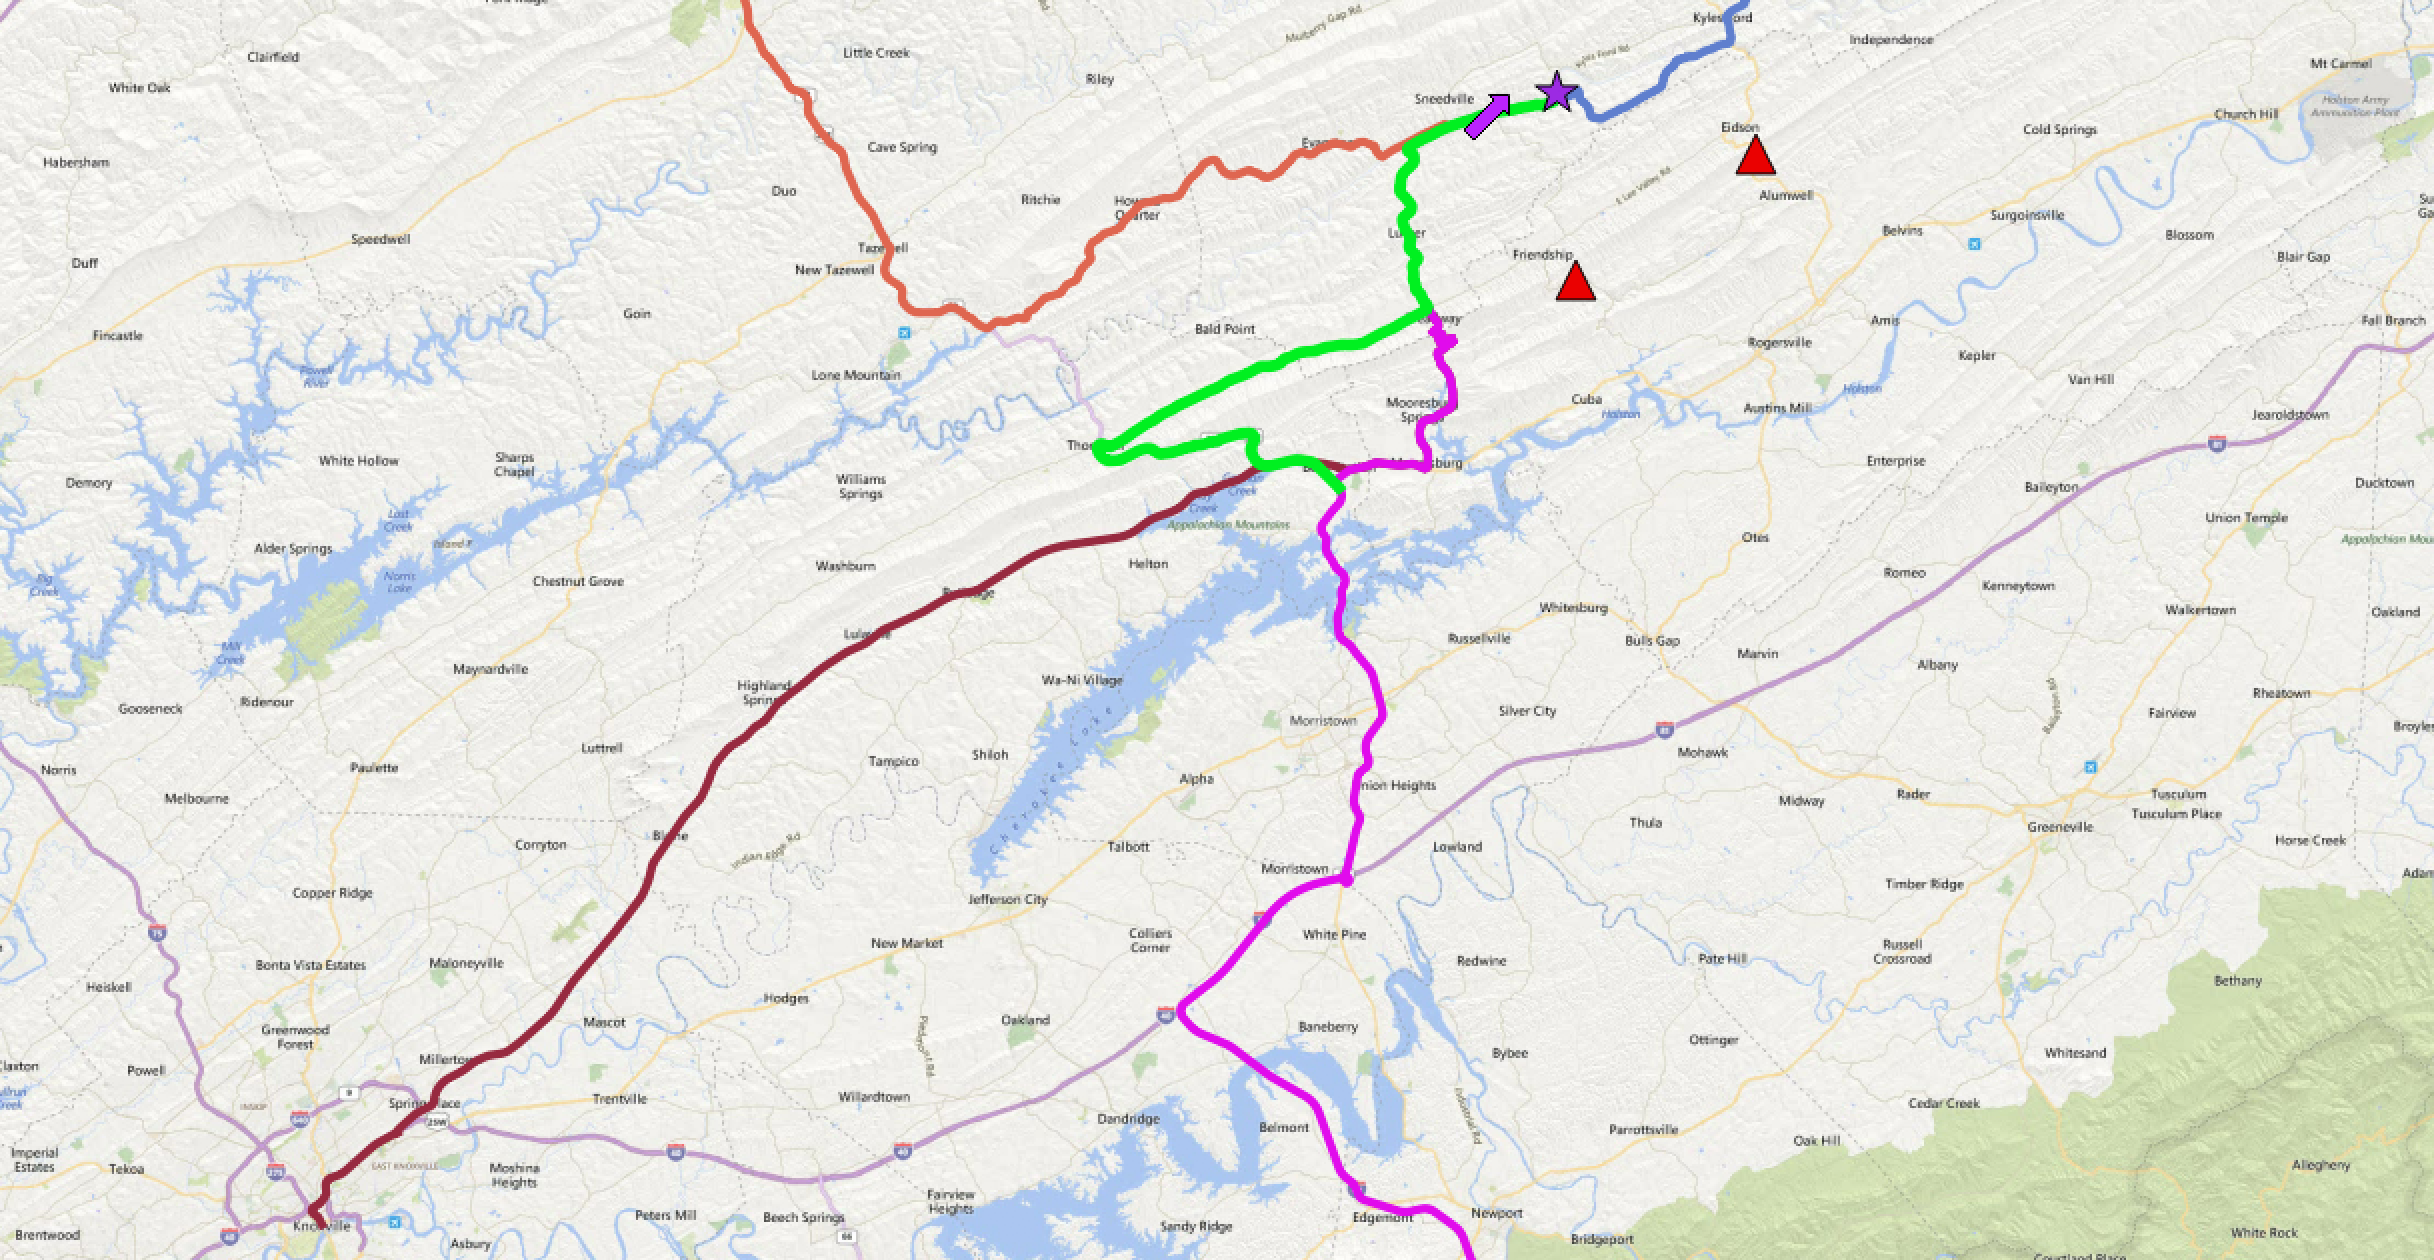
\includegraphics[width=\textwidth]{images/overviewMap.png}
\caption{Getting to the landing site. The colored-in routes are described in the following sections. Close-ups of the Bean Station and Sneedville areas can be found below. Please note that the road is closed where the red blobs are!!}
\label{image:overviewmap}
\end{sidewaysfigure}

\begin{figure}[H]
\centering
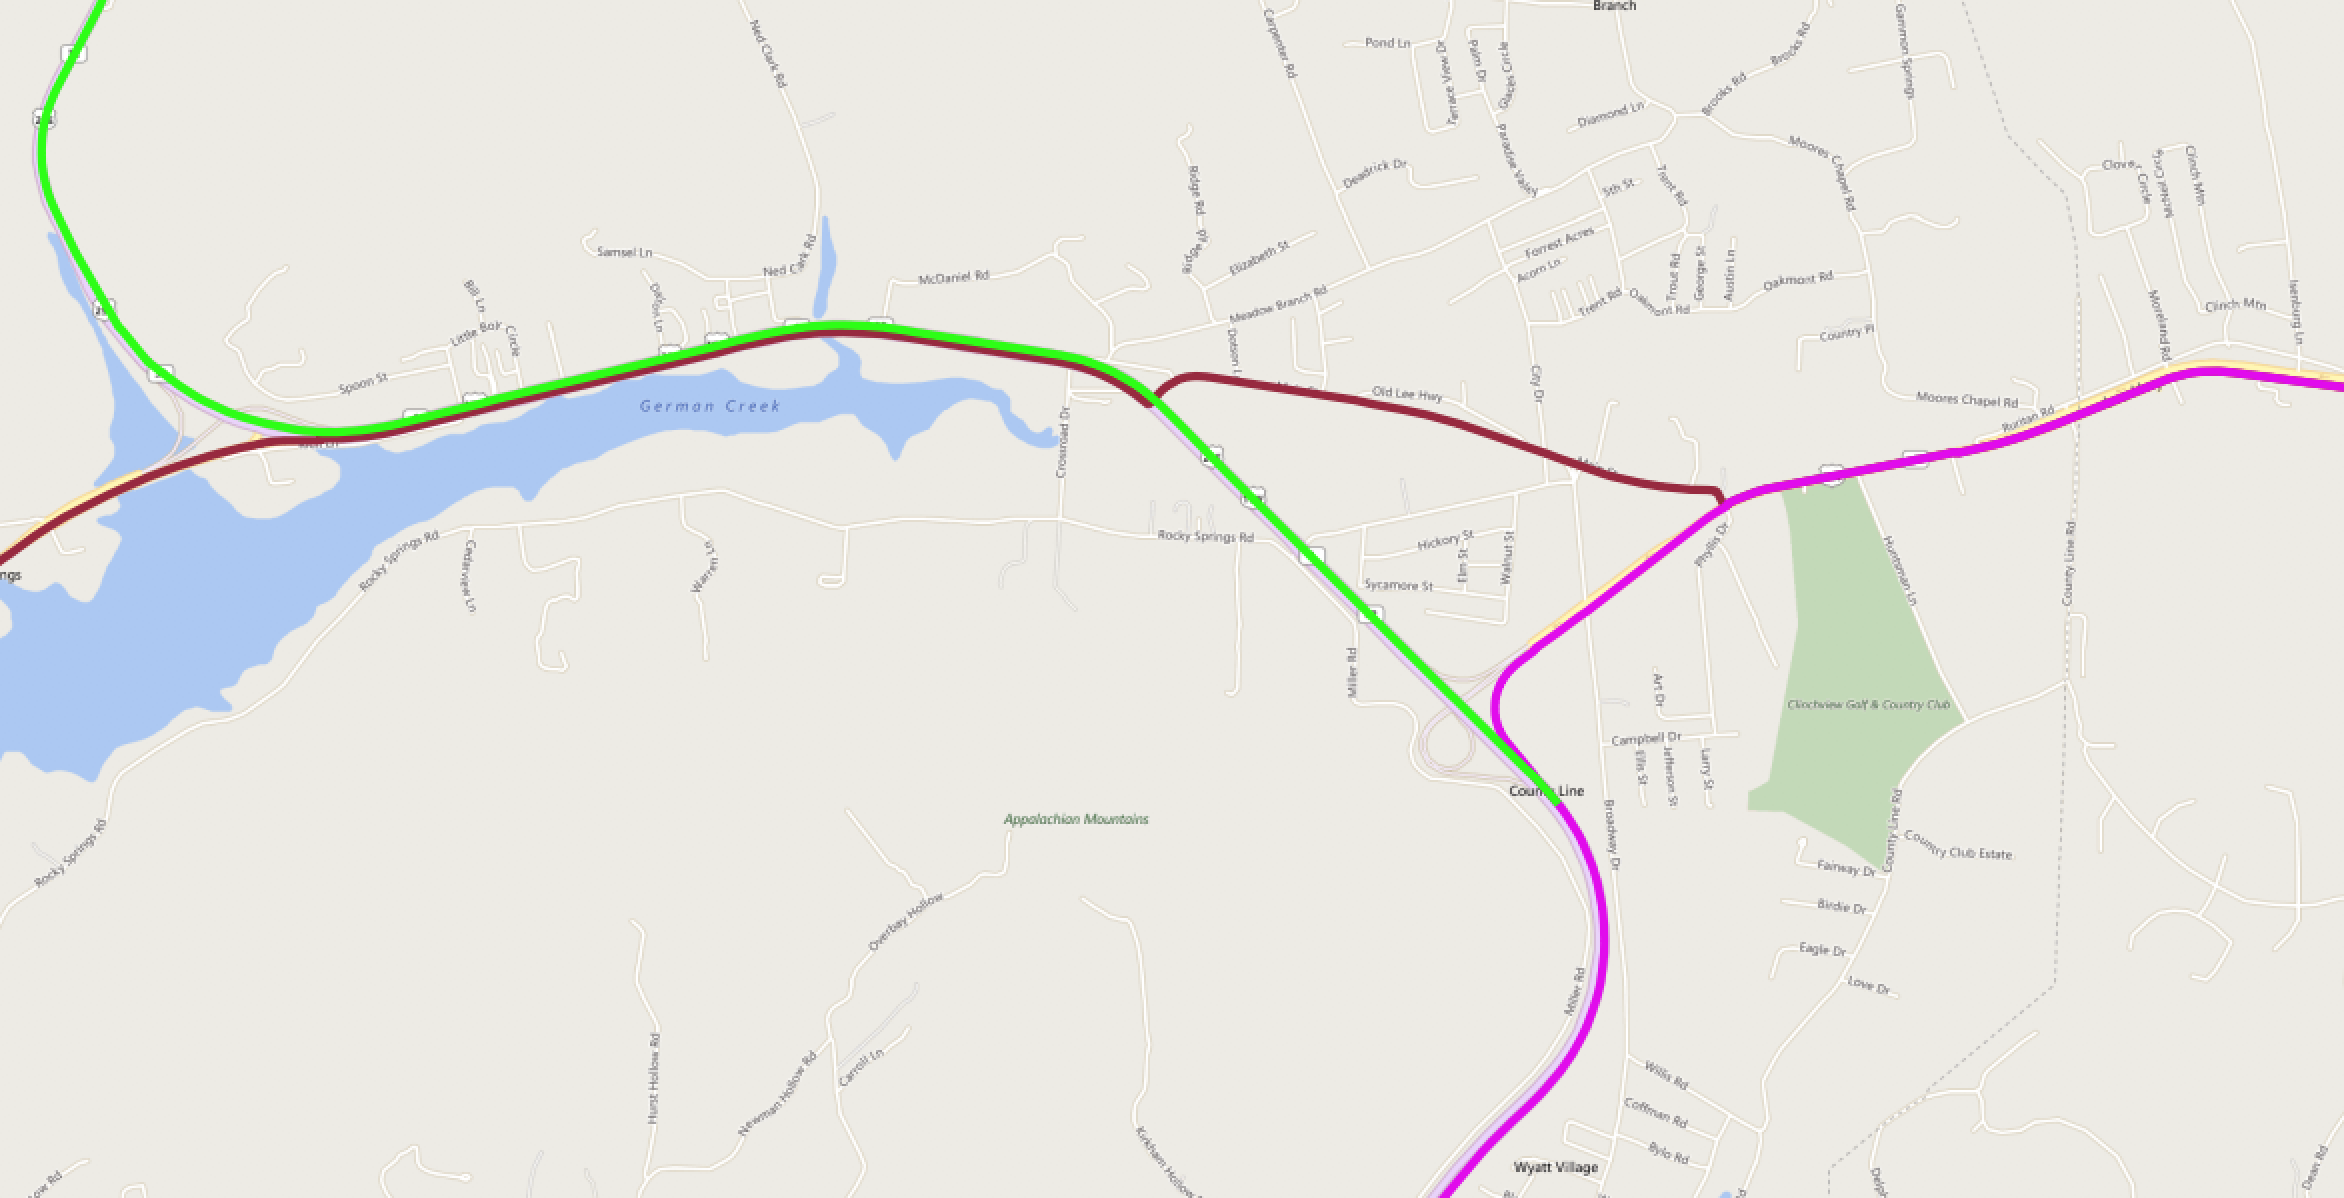
\includegraphics[width=.9\textwidth]{images/overviewBeanStation.png}
\caption{Close-up of the Bean Station area. Crew from the Knoxville and Asheville direction will have to navigate this area. The bright green route is the struggle-free route.}
\label{image:beanstation}
\end{figure}
\vfill
\begin{figure}[H]
\centering
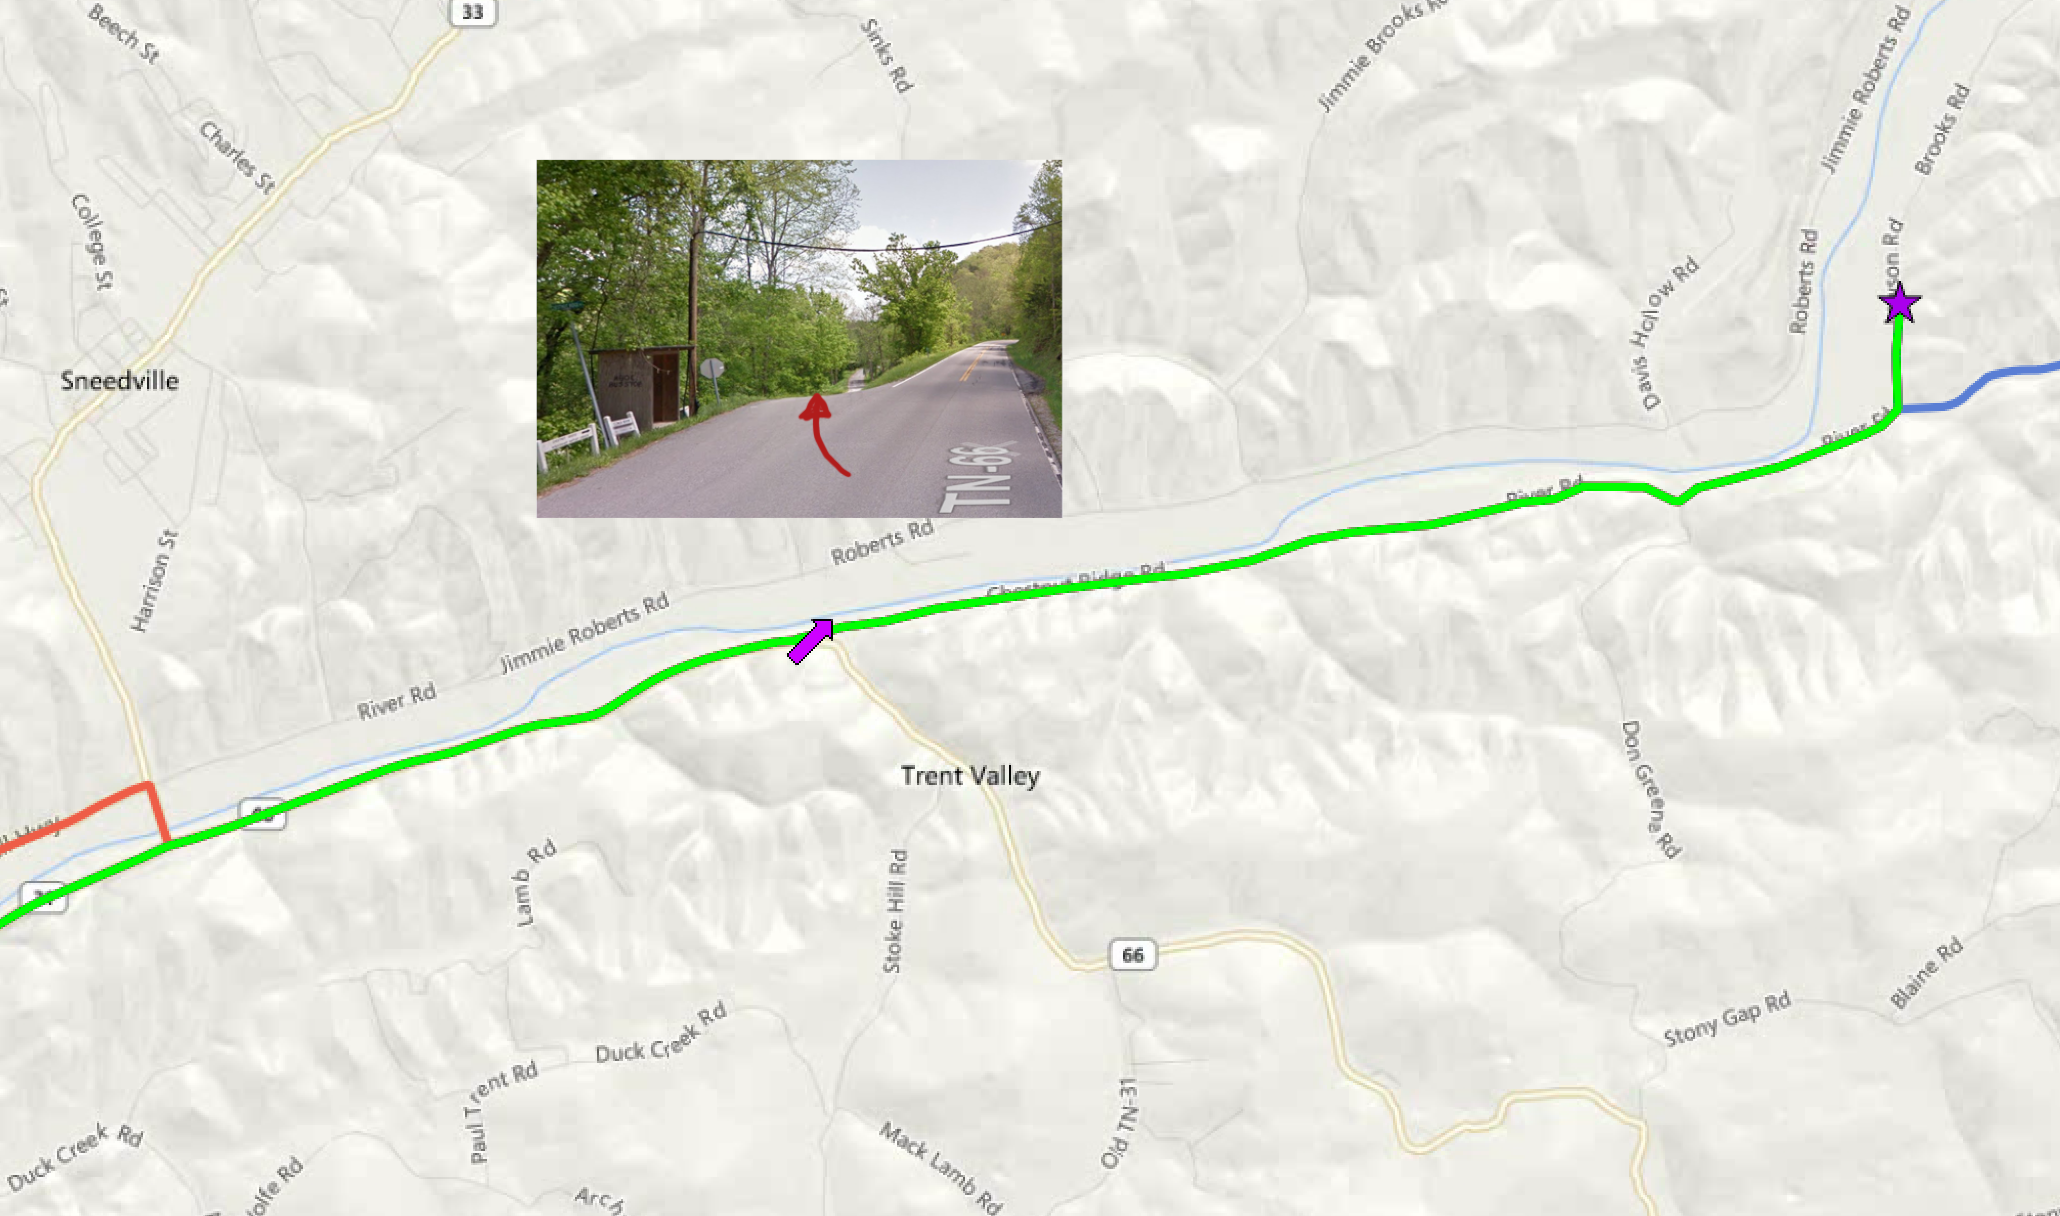
\includegraphics[width=.9\textwidth]{images/overviewTTMSite.png}
\caption{Close-up of the Sneedville area and the Landing Site. Crew from all directions will have to navigate this area. Please pay special attention to the highlighted fork -- you'll want to keep left!}
\label{image:sneedville}
\end{figure}
% {\centering\label{image:overviewmap} 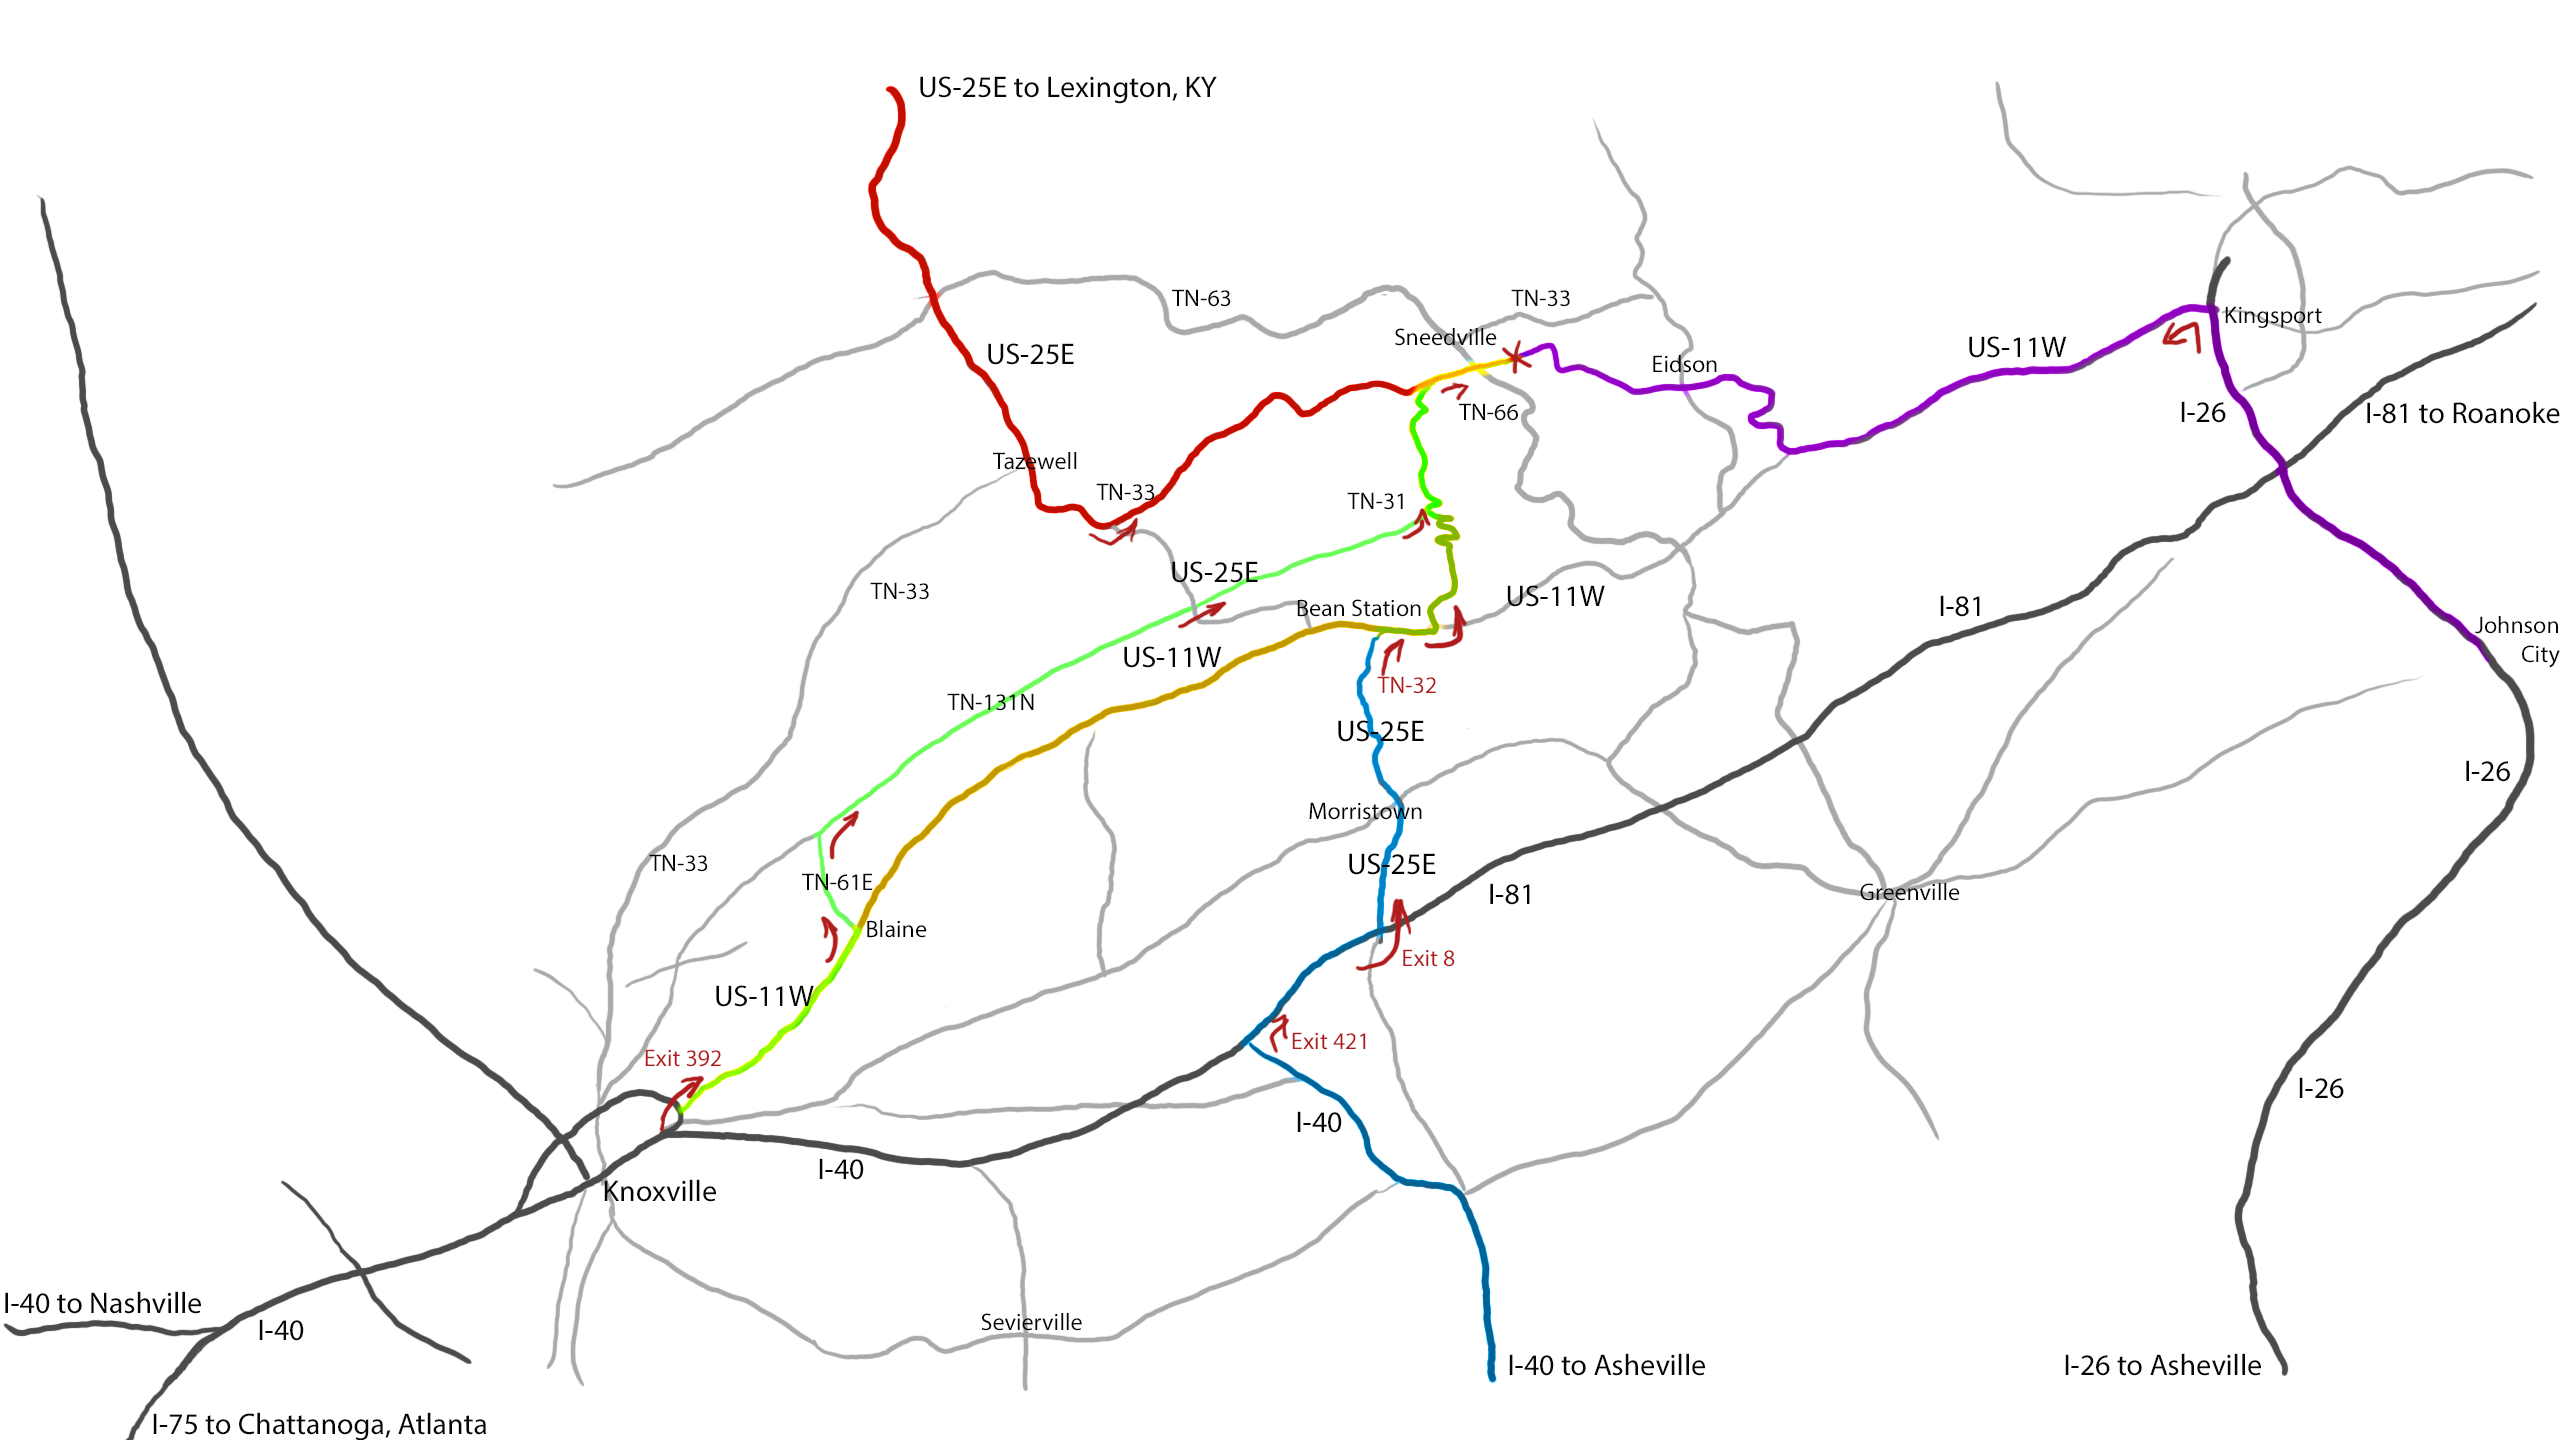
\includegraphics[height=\textheight]{images/maptosite_highlighted.png}}
% {\centering\label{image:beanstation}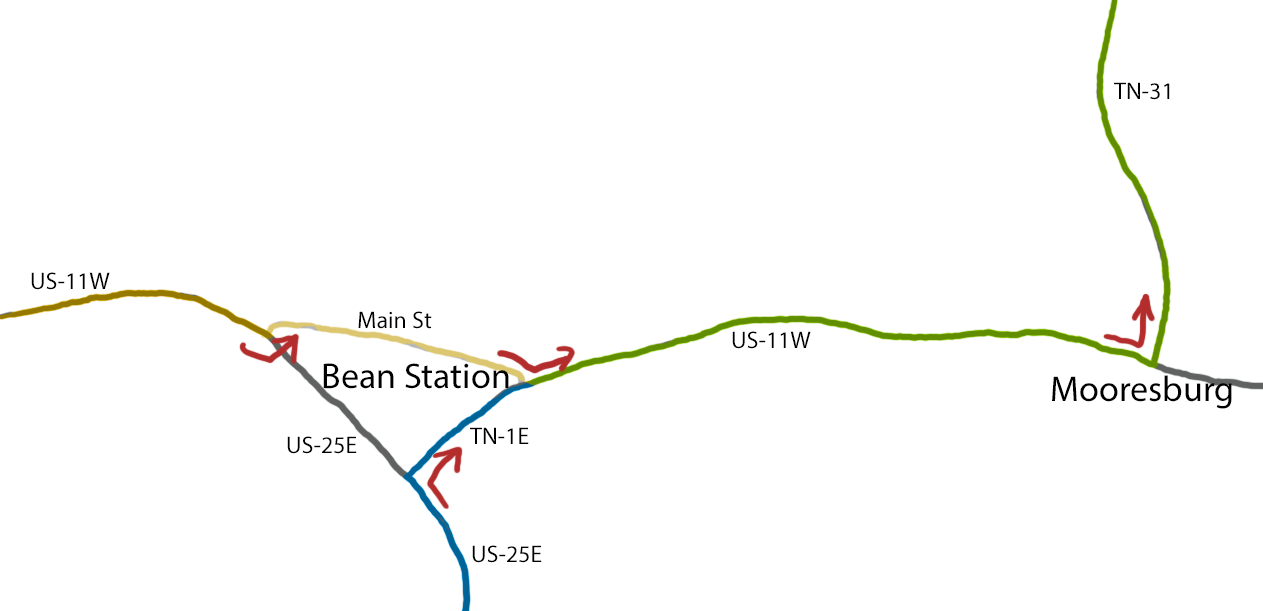
\includegraphics[width=\textwidth]{images/beanstationmap-highlighted.png}}
% \vfill
% {\centering\label{image:sneedville}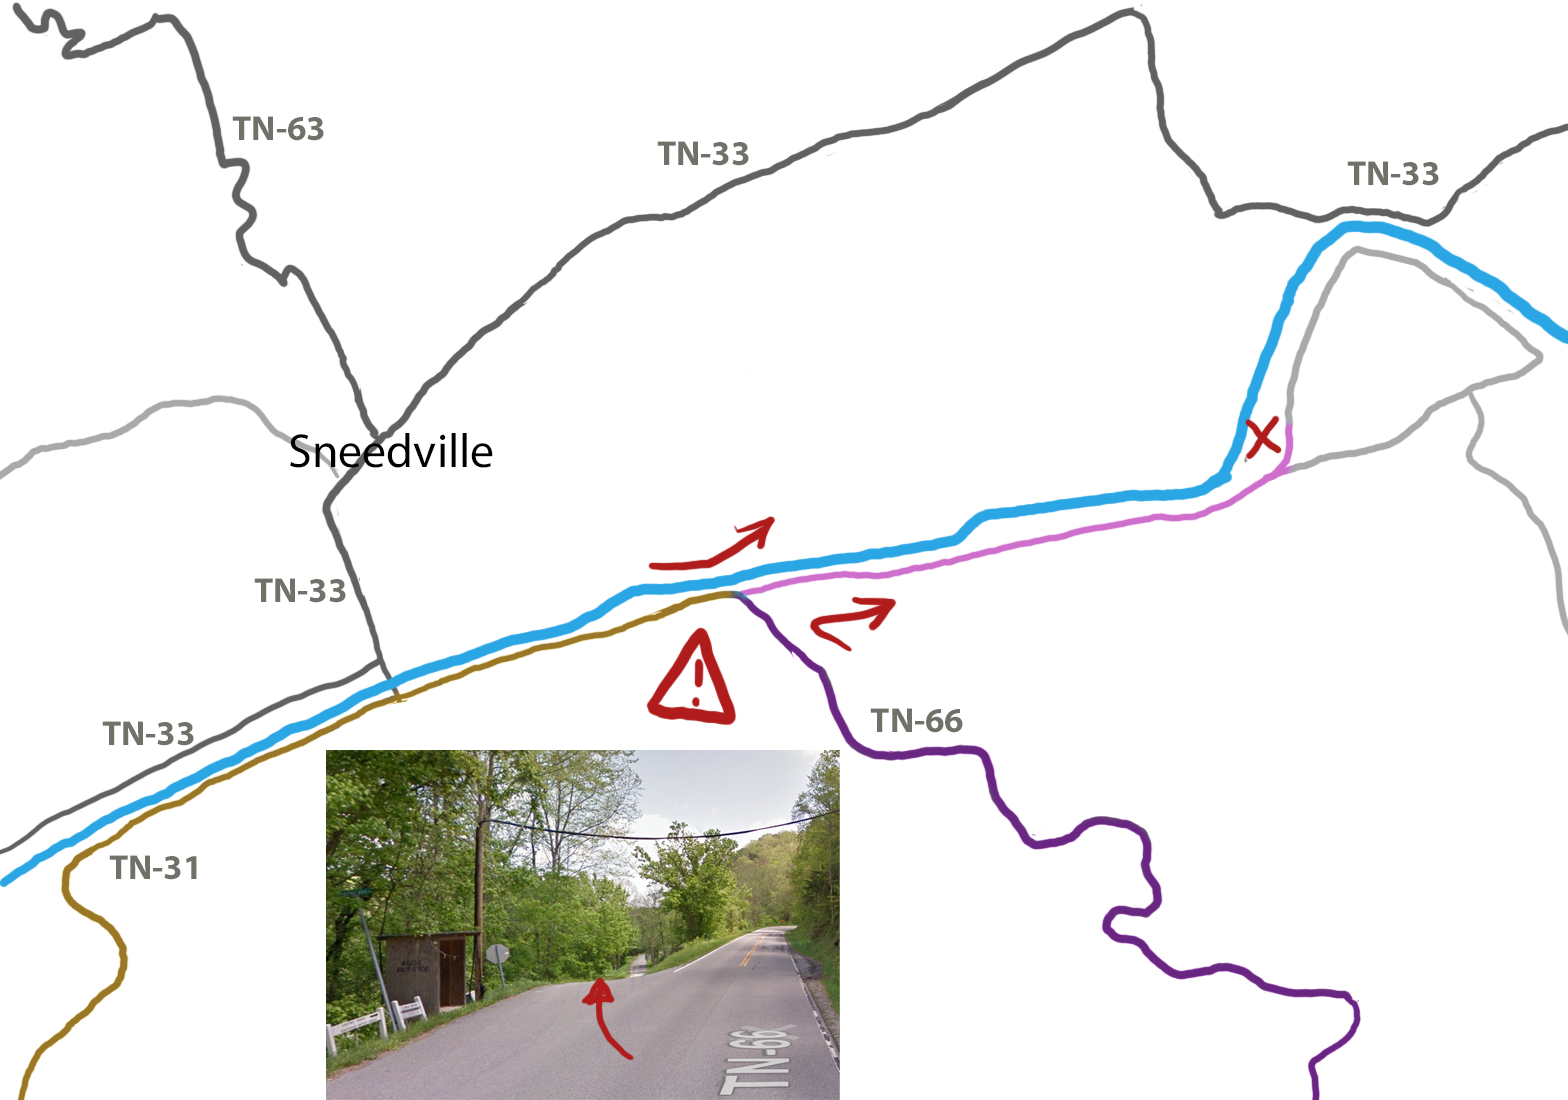
\includegraphics[width=\textwidth]{images/sneedville-closeup-highlighted.png}}

\subsection*{Flight Path}
A map of the flight path can be found on page \pageref{image:overviewmap}.
% \begin{wrapfigure}{R}{0.3\textwidth}
% \centering
% 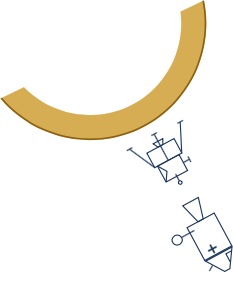
\includegraphics[width=0.25\textwidth]{images/landing1.png}
% % \caption{}
% \end{wrapfigure}

Due to road closures, we have to re-write the written instructions.
In the meantime, feel free to check out this interactive map \url{https://drive.google.com/open?id=1sqBiYj6TCQhonnQ6H-CkACDfmJQqir_r&usp=sharing}.

\todo[inline]{rewrite instructions}
\subsubsection*{Struggle-Free Route (Green)}
The fastest routes to Spirit Crossing are full of switchbacks to avoid various objects in orbit. If you don't mind dodging the odd satellite, you can find instructions that suit your agile rocket needs. If your spaceship is rather large or you haul a shuttle, we recommend the struggle-free route. You can find this route on the maps highlighted in green.

\begin{enumerate}[noitemsep]
	\item From Knoxville: Follow directions until \ref{us11w}.
	\begin{enumerate}
	    \item After passing through Tate Springs, you will turn left onto TN-32N.
	\end{enumerate}
    \item From Asheville:
    \begin{enumerate}
        \item Instead of turning right in Bean Station, you will follow signs for TN-32N.
    \end{enumerate}
    \item After about 7.5 miles, turn right onto TN-131N (Mountain Valley Highway). 
    \item About 13 miles later, turn left onto TN-31N.
    \item Stay on TN-31N for 8.5 miles. Then, continue from step \# \ref{dir:chestnutridge} in the ``From Knoxville'' directions.
\end{enumerate}

\subsubsection*{From Knoxville and points Southwest (Yellow)}
You can find this route on the maps highlighted in yellow.

\begin{enumerate}[noitemsep]
	\item Take I-40 E from downtown Knoxville.
    \item Take exit 392 for US 11W N/Rutledge Pike/Knoxville Zoo.
    \item Continue 40 miles to merge right onto US 11W / Hwy 25 E. \label{us11w}
    \begin{enumerate}
        \item For the struggle-free route, you will turn left onto TN-32N after passing through Tate Springs (about a mile before Bean Station) and follow along from step \ref{strugglefree}.
    \end{enumerate}
    \item After about a mile, turn left on to Main St.  You should see a red store on the left. A close-up of this area can be found on page \pageref{image:beanstation}.
    \item In about two miles, turn left on to US 11W.
    \item After about 2.8 miles, turn left on to TN 31.  There will be an Exxon station on the left at the intersection. \label{dir:tn31}
    \item Drive for about 17 miles and then continue straight on to TN 66 S.
    \item Drive 1.4 miles for slight left onto Chestnut Ridge Road.  Look for the ``To the Moon'' sign along the road; \textbf{this is a tricky intersection that's easy to miss. \label{dir:chestnutridge} You can find a picture and close-up of this area in the Sneedville area map on page \pageref{image:sneedville}}
    \item After about \sfrac{1}{3} of a mile, turn left on to Clinch River Circle
    \item Welcome home!  Please follow instructions in the next section, ``Landing Procedure,'' on page \pageref{sec:parking}
\end{enumerate}


% \clearpage
\subsubsection*{From Asheville and points Southeast (Blue)}
You can find this route on the maps highlighted in blue.

\begin{enumerate}[noitemsep]
	\item Take I-40 W to I-81
    \item Take exit 8 for US 25 E towards Morristown/White Pine
    \item Take exit to 11W north towards Rogersville
    \item In Bean Station, continue on TN-1 E/TN-32 N. A close-up of this area can be found on page \pageref{image:beanstation}.
    \begin{itemize}
        \item For the struggle-free route, follow signs for TN-32N.
    \end{itemize}
    \item Continue from step \# \ref{dir:tn31} in the ``From Knoxville'' directions
\end{enumerate}


\subsubsection*{From Johnson City and points East (Dark Pink)}
You can find this route on the maps highlighted in dark pink.  Note that this routes around TN-66 near Spruce Pine Road and TN-70 near Cave Springs Rd that are closed due to mud-slides.  If relying on your own navigation system, please be aware that you cannot use these roads.  (Though, if coming from Johnson City, TN-70 should be OK for coming the final stretch as that is well above the mudslide.)

\begin{enumerate}[noitemsep]
	\item Take I-26W
    \item Continue on US23 through Kingsport
    \item US23 turns into US23/58 in Weber City, Virginia; stay on US23/58.
    \item Turn left onto VA-600/VA-623; Continue to follow VA-600
    \item Continue straight onto VA-696 entering Tennessee
    \item Continue on TN-33 S
    \item Turn left on TN-70 S
    \item Turn right on Chestnut Ridge Road. This is a steep turn! You can find a picture and close-up of this area in the Sneedville area map on page \pageref{image:sneedville}
    \item Turn right on Clinch River Circle
    \item Welcome home!  Please follow instructions in the next section, ``Landing Procedure,'' on page \pageref{sec:parking}
\end{enumerate}


\subsubsection*{From Lexington, KY and points North (Red)}
You can find this route on the maps highlighted in red.

\begin{enumerate}[noitemsep]
	\item Take I-75 S
    \item Take exit 29 for US-25E, turn left onto US-25E
    \item Turn left onto TN-33 N
    \item Turn right onto TN-31 S/TN-66 S
    \item Turn left onto TN-66 S
    \item Resume from step \# \ref{dir:chestnutridge} in the ``From Knoxville'' directions
\end{enumerate}

\section*{\Gls{gate} Hours}
\label{sec:gate}

Please see Table \ref{tbl:gatehours} on page \pageref{tbl:gatehours} for a detailed list of gate hours.

\Gls{gate} is closed during and after Effigy and Temple Burn

\textbf{** No admission after 6 p.m. Saturday **}
 
All unused tickets are void after 6pm Saturday and the burn is closed for entry. 

\textbf{** Absolutely no ticket sales at the gate **}

% \clearpage

\section*{Landing Procedure}
\label{sec:parking}

% \bod[inline]{This will have to be vetted and expanded by gate and/or BoD}

\begin{enumerate}[noitemsep]
	\item arrive at Spirit Crossing entrance where \gls{parking} volunteers will navigate you to a staging area for check-in
    \item check-in at \gls{gate} with tickets and ID
    \item receive wrist-band; keep this wrist-band with you at all times (please see page \pageref{sub:wristbands} for more information on wristband policy)
    \item proceed to \glspl{greeter} to be properly welcomed and oriented -- be sure to get your swag!
 	\item offload equipment at your deployment site
      \begin{itemize}
          \item If you are driving an RV or using a camper
              \begin{quote}
                  \gls{parking} will direct you to your final deployment area for RVs and campers
              \end{quote}
          \item If you are driving a regular vehicle
              \begin{itemize}
          		\item If this is a \gls{mudburn}
              		\begin{quote}
              			if the site is too muddy for vehicles, you may have to hoof in your gear; or, coordinate with the \gls{gate} on asking \gls{love} to shuttle your gear to your site
              		\end{quote}
          		\item If the grounds are driveable
              		\begin{enumerate}
                       \item Since there is limited access on-site for bringing vehicles for offloading coordinate with \gls{gate} for getting an offloading pass 
                       \item drive to site
                       \item offload gear (do NOT take the time to set up!)
                       \item drive back to \gls{gate} to return offload pass
                    \end{enumerate}
                \item If you arrive after dark (regardless of weather conditions), \gls{love} will shuttle participants' belongings from the \gls{gate} to their camps, eliminating the presence of burner blinding non-art cars freely roaming the burn field.
             \end{itemize}
      \end{itemize}
    \item return to \gls{parking} to properly land vehicle for event duration
    \item finish deploying your gear at your camping site
%      \item go to \gls{parking} to land vehicle into assigned landing pad
%     \item check-in with \gls{gate} that you have offloaded
\end{enumerate}

\vfill
\begin{figure}[H]
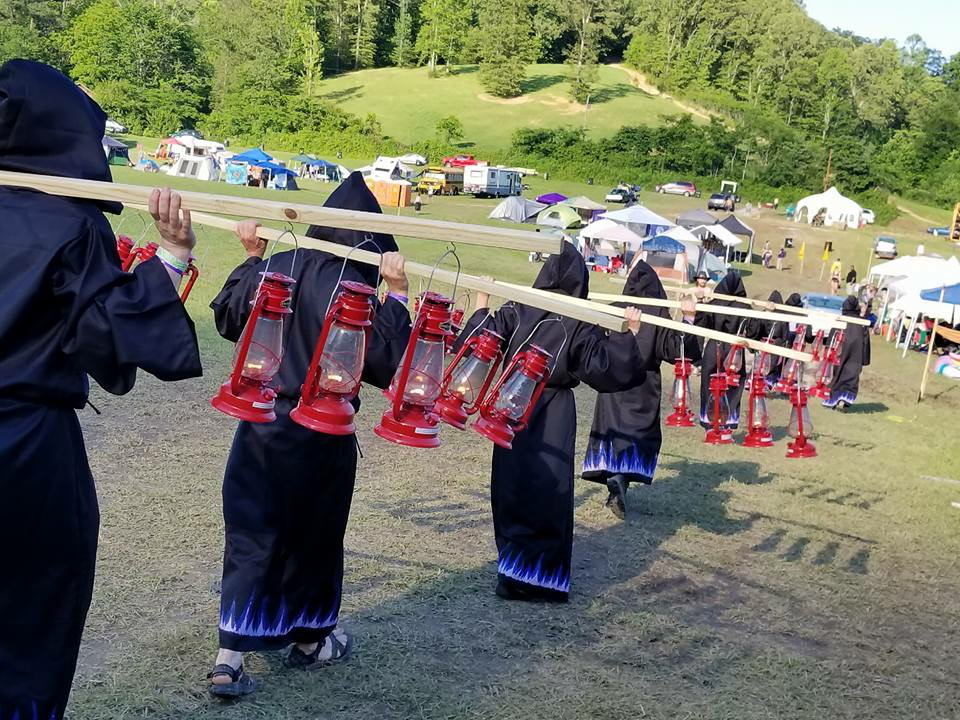
\includegraphics[width=\textwidth]{images/lamplighters.jpeg}
\caption{Lamplighters at work. Image courtesy of Johnny “Twaffle” Benton, 2017.}
\label{fig:lamplighters2017}
\end{figure}

\chapter{In-Flight Procedures}

% This is true if only doing the flight manual, not the pre-flight
\ifisflight
  % This one page needs to be one column to look right, even
  % in the flight manual, proper.
  % failed experiment to add thumb guides
%   \addthumb{Welcome}{}{white}{black}
\putchapterthumb
\fi


Once you're at \gls{ttm}, you'll want to keep gate hours in mind (if you leave), and before you finally pack up to go to your rest-of-the-year home, please take a moment to read through our takeoff procedure!

\section*{Gate Hours}

\textbf{No vehicles will be allowed in after sunset! No moving vehicles \textit{period} inside the burn when it's dark - so if you get there right before sunset, you better get in, unload your stuff, and get right back out to parking ASAP. This is for the safety of everyone at the burn!}

Any vehicles that arrive after sunset will be redirected to parking, where we may or may not have a golf cart to help you carry some stuff in --- but don't count on it --- use that Radical Self-Reliance!

\begin{table*}[h!]
\footnotesize
\centering
\caption{\Gls{ttm} \gls{gate} hours}
\label{tbl:gatehours}
\begin{tabular}{@{}lll@{}}
\toprule
Wednesday & 6/12/2019 & 12--10\pm EST                                    \\ 
          &           & Theme Camp Early Entry Only w/ Pre-Registration \\
Thursday  & 6/13/2019 & 10\am--12\am EST                                   \\
Friday    & 6/14/2019 & 10\am--12\am EST                                    \\
Saturday  & 6/15/2019 & 10\am--6\pm EST, no admission after 6pm for rest of event \\
Sunday    & 6/16/2019 & 10\am--6\pm EST                                    \\
          &           & Departing Only                                  \\
Monday    & 6/17/2019 & 8\am--12\pm EST                                    \\
          &           & Departing Only                                  \\ \bottomrule
\end{tabular}
\end{table*}

\section*{Re-entry Procedure}

\textbf{There is no after hours entry without pre-arranged permission.  Crew arriving at the site outside gate operating hours will be turned away.  No crew is permitted to wait on the property until the gate opens.}

Please contact the \gls{bod} via \url{connect@tothemooonburn.com} well in advance of the event to work out options if long-distance travelers cannot arrive while the gate is open.

For the safety of other patrons and to preserve the integrity of the experience, \textbf{no} coming and going at leisure is allowed after checking in.  Exiting and returning \gls{ttm} are reserved \textbf{for medical and emergency reasons only}, and must be communicated to and cleared by the Gate Lead prior to leaving.

Theme Camp supply runs are possible Wednesday -- Friday before 10\pm \textbf{only}. Before leaving, \textbf{check at the gate} if a pass is needed. The Gate will check with \Gls{el} on call and a re-entry lanyard will be issued at \gls{el} discretion.

% If you forget something and need to ``make a run to the store'' talk to a team / event  / gate lead and we can grant Re-Entry if you combine your trip with one beneficial \gls{ttm} and the community at large.

\section*{Takeoff Procedure}
\subsection*{Leave No Trace}
\Gls{ttm} follows the \gls{lnt} principle (see \gls{tenprinciples}, page \pageref{tenprinciples}). Please take all your belongings, trash, and \gls{graywater} with you and leave the site in a better shape than you found it.

\subsection*{Takeoff Launch Window}

\Gls{ttm} officially closes at 11:59\pm EST, Sunday, June 17th.  All crew must vacate the site by 12pm EST, Monday, June 18th unless given explicit prior permission from Theme Camp Late Departure.

Vehicles can be driven on site on Monday to pack up. In case of inclement weather, a no driving / limited access policy to site will be implemented. Be prepared by bringing your own cart / wagon to transport gear out and to your vehicle.
\Gls{love} will be able to assist with shuttling gear to parking. 
Vehicles can \textbf{not} be parked alongside road to do so, but only be lined up at gate about 10 at a time.

Pleases look for announcements at \Gls{cockpit} / \Gls{gate}, as this policy may slightly change, depending on situation. 

\newpage
\section*{Resources}

% \begin{wrapfigure}{R}{0.3\textwidth}[h!]
% \centering
% 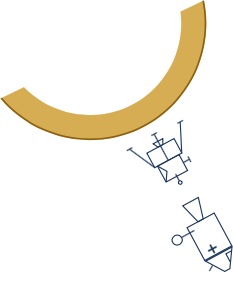
\includegraphics[width=0.25\textwidth]{images/landing1.png}
% % \caption{}
% \end{wrapfigure}
% \begin{multicols}{2}
\subsection*{Showers}
There are no showers. To keep yourself clean, bring wet wipes or biodegradable soap.
Please don't clean your dishes or yourself in the river since there are mussels in the river that are protected wildlife.  (And these are also the reason you should wear river shoes while in the river as the mussels will cut you. They're mean that way.)

\subsection*{Ice}
Ice will be soled from noon to 3 \pm every day for \$2 per 10 lbs bag.  Cash only! Bring small bills please. 


\subsection*{Lost and Found}
The Lost and Found will be at the \gls{cockpit} / \gls{vc} station.

\subsection*{Port-a-Potties}
There are Port-a-Potties on-site. Please don't put anything other than one-ply toilet paper and human waste in the Port-a-Potties. You will find Port-a-Potties in multiple locations across the site.



% \reflectbox{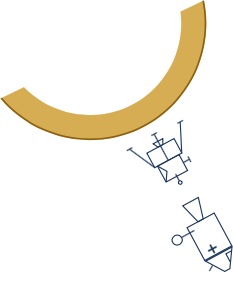
\includegraphics[width=\columnwidth,angle=180]{images/landing1.png}}

% \vspace*{\fill}
\ifisflight
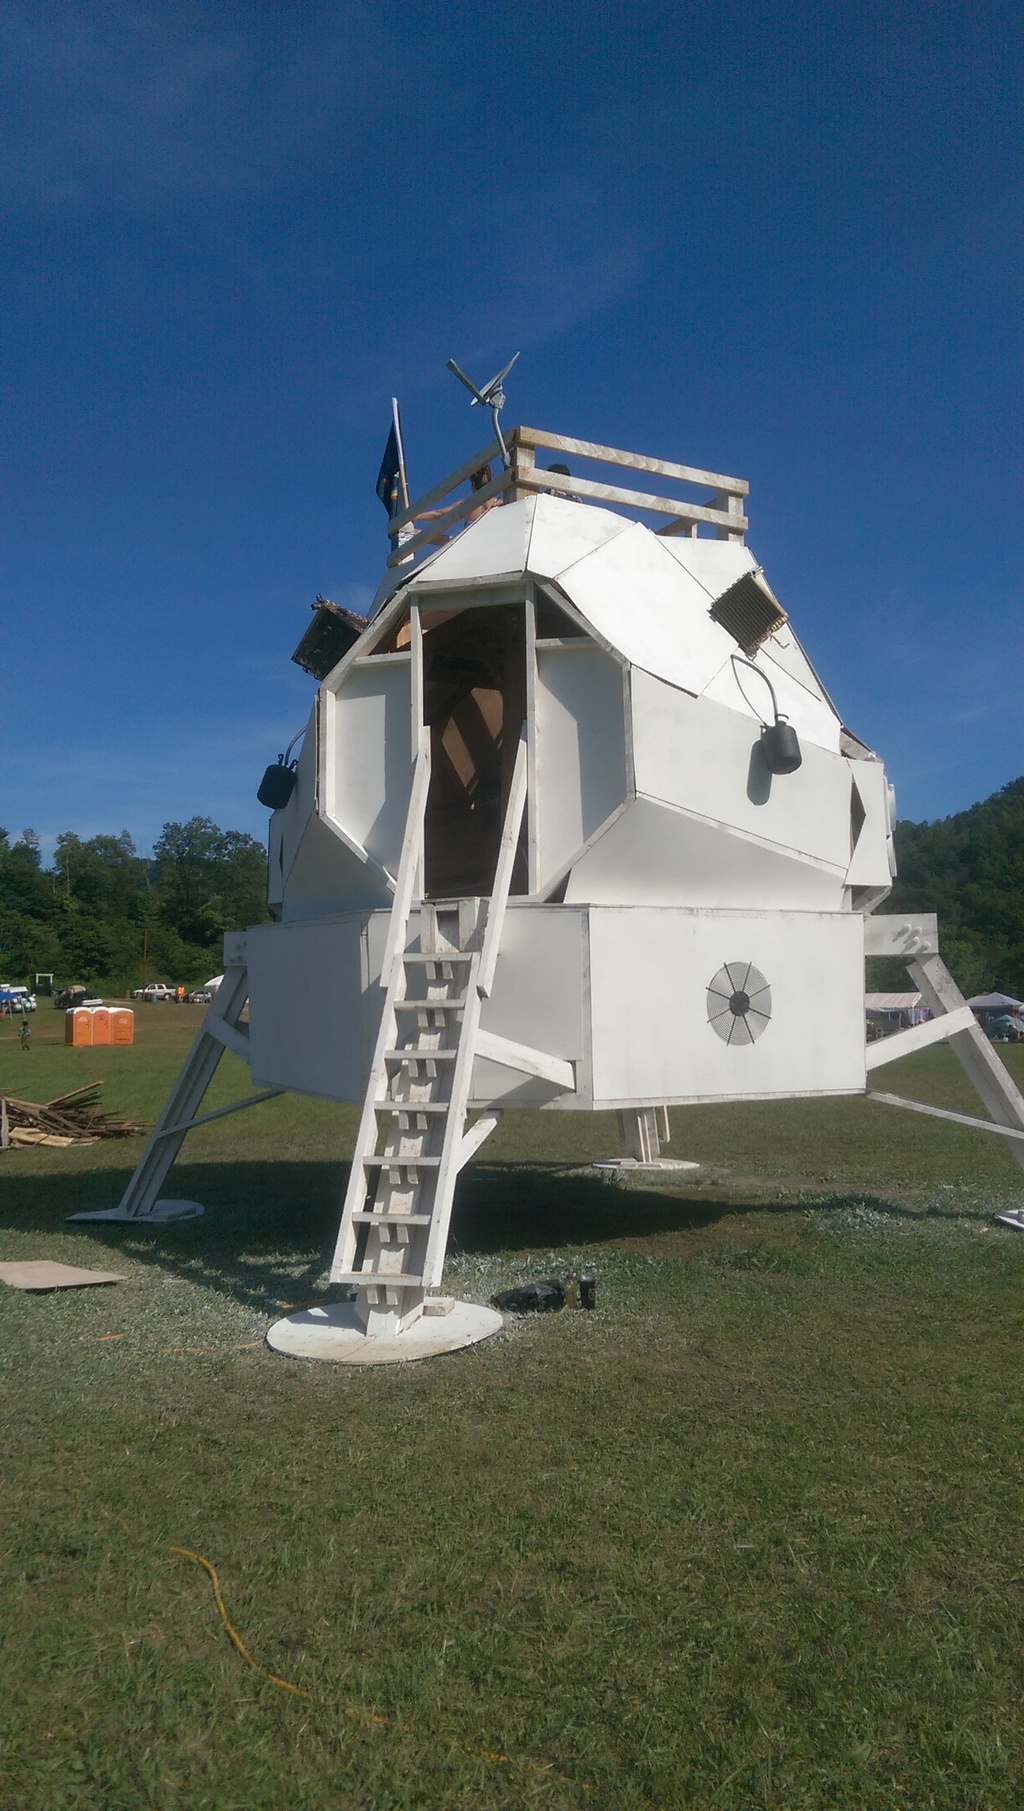
\includegraphics[width=\columnwidth]{images/2017Effigy_small.jpg}
\fi

% \section{Where to camp}
% \missingfigure{Site map highlighting approved camping areas }

% \section{Crew Restricted Areas}
% \missingfigure{Site map highlighting public vs crew only areas}


% \section{Pre-flight Procedures}
\section*{Crew Equipment}
% Things to do / pack before leaving
\gls{ttm} is an exercise in radical self-reliance.  This means bringing everything you are going to need, which includes food, water, shelter, any medications, and hygiene products.  You must take responsibility for your own well-being and survival.  Do not expect the community to take care of you.  Though there are EMTs on site, they are only an emergency resource, so do not rely on them for basic over-the-counter medications.

\subsection*{Crew Inventory Checklist}
Below is a list of items we suggest you bring with you.  A burn requires a certain amount of preparation to be able to sustain you for 4--5 days of camping with minimal amenities. Please come prepared.  While this isn't the Playa, the nearest store is a bit removed so pack what you need and extra.  

% The following are checklists for items that are recommended to bring to ensure maximum likelihood of survival and an otherwise hoopilicious time.  The first checklist is for items that crew should bring; the second are for nice to have items.

\subsubsection*{Must Haves}

\begin{multicols}{2}

\begin{checklist}
	\item \textbf{A valid, state-issued} photo ID
    \item Your printed ticket
    \item Emergency contact
    \item 1 gallon of water per person per day!  Spirit Crossing does not provide water but does have a well accessible if needed - bring your own. In case of shortage, a hose is available for filling up but please plan ahead!
\end{checklist}
\end{multicols}

\subsubsection*{Strongly Recommended}

\begin{multicols}{2}

\begin{checklist}
	\item tent
    \item sleeping bag and/or bedding
    \item blankets
    \item tarps
    \item 3 gallons of water per person per day for drinking, washing, and food preparation
    \item food for everyone in your group for length of stay
    \item sufficient ice for duration \footnote{Some stores also sell dry ice. However, be sure to wrap dry ice in towel for further insulation.}
    \item any necessary medication
    \item epi pen
    \item if needed, contact lens supplies
    \item first aid kit
    \item sunblock
    \item insect repellent
    \item deodorant
    \item single ply toilet paper \footnote{The port-a-potties only get serviced once a day, and may run out of toilet paper.}
    \item paper towels
    \item baby wipes or moist towelettes
    \item towels
    \item biodegradeable body washing soap \footnote{Please do not wash in the river.}
    \item biodegradeable dishwashing soap \footnote{Do not wash dishes in the river, and exercise proper gray water management.}
    \item \gls{graywater} container and funnel \footnote{A cat litter bucket works well as gray water containment.}
    \item garbage bags, recycling bags, and tools for \gls{moop} containment
    \item flashlights, spare batteries, headlamps, LEDs for your camp  (solar powered recommended) 
    \item reusable cup or bottle \footnote{Many camps offer drinks, but do not provide cups.  A cup with a carabiner is ideal.}
    \item reusable utensils and dinnerware \footnote{Many camps offer food, but do not provide utensils or plates}
    \item condoms
    \item pocket knife
    \item hammer
    \item sunglasses
    \item rain hat / rain gear / umbrellas
    \item gifts
    \item a loving and open mind
    \item \hrulefill
\end{checklist}

% * <mcoletti@gmail.com> 2018-05-08T17:10:50.436Z:
% 
% >     \item \hrulefill
% Possibly add more of these to fill out the page.
% 
% ^.\

\end{multicols}

\subsubsection*{Optional}

\begin{multicols}{2}

\begin{checklist}
    \item swimsuit
    \item water shoes
    \item inner-tube
    \item can or bottle opener
    \item simple toolkit
    \item rubber mallet
    \item rope, string, zip ties, duct tape
    \item sewing kit
    \item portable metal ashtrays \footnote{Mint tins work well for this purpose.}
    \item lawn chairs
    \item pop-up shelters, pavilions, or other forms of portable shelter
    \item ice chests
    \item camp cooking stove
    \item fuel for stove 
    \item fire bowl
    \item fire wood
    \item fire extinguishers
    \item fuel and safety gear for fire performance
    \item watertight protective bags \footnote{For cameras and electronics.}
    \item generator
    \item tea and/or coffee
    \item coffee pot, tea pot, or french press
    \item earplugs
    \item musical instruments
    \item parasols
	\item spray bottle of water for keeping cool
    \item pasties 
\end{checklist}

\end{multicols}


\subsection*{Prohibited Items} %\todo{themed name?}
Please do not bring \textbf{any} of the following items:

\begin{multicols}{2}
\begin{itemize}[noitemsep]
	\item Handheld lasers --- they are too powerful to be safe
    \item Fireworks --- unsafe use of fire and creates \gls{moop}
    \item Chinese/fire lanterns --- uncontrollable, flaming \gls{moop} 
    \item Pets of any kind (please see pets policy on page \pageref{sub:nopets})
\end{itemize}
\end{multicols}

\newpage
\section*{Resources}

% \begin{wrapfigure}{R}{0.3\textwidth}[h!]
% \centering
% 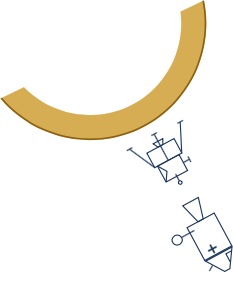
\includegraphics[width=0.25\textwidth]{images/landing1.png}
% % \caption{}
% \end{wrapfigure}
% \begin{multicols}{2}
\subsection*{Showers}
There are no showers. To keep yourself clean, bring wet wipes or biodegradable soap.
Please don't clean your dishes or yourself in the river since there are mussels in the river that are protected wildlife.  (And these are also the reason you should wear river shoes while in the river as the mussels will cut you. They're mean that way.)

\subsection*{Ice}
Ice will be soled from noon to 3 \pm every day for \$2 per 10 lbs bag.  Cash only! Bring small bills please. 


\subsection*{Lost and Found}
The Lost and Found will be at the \gls{cockpit} / \gls{vc} station.

\subsection*{Port-a-Potties}
There are Port-a-Potties on-site. Please don't put anything other than one-ply toilet paper and human waste in the Port-a-Potties. You will find Port-a-Potties in multiple locations across the site.



% \reflectbox{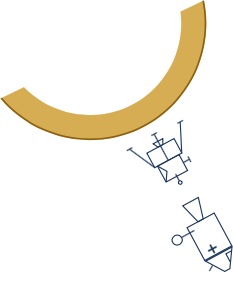
\includegraphics[width=\columnwidth,angle=180]{images/landing1.png}}

% \vspace*{\fill}
\ifisflight
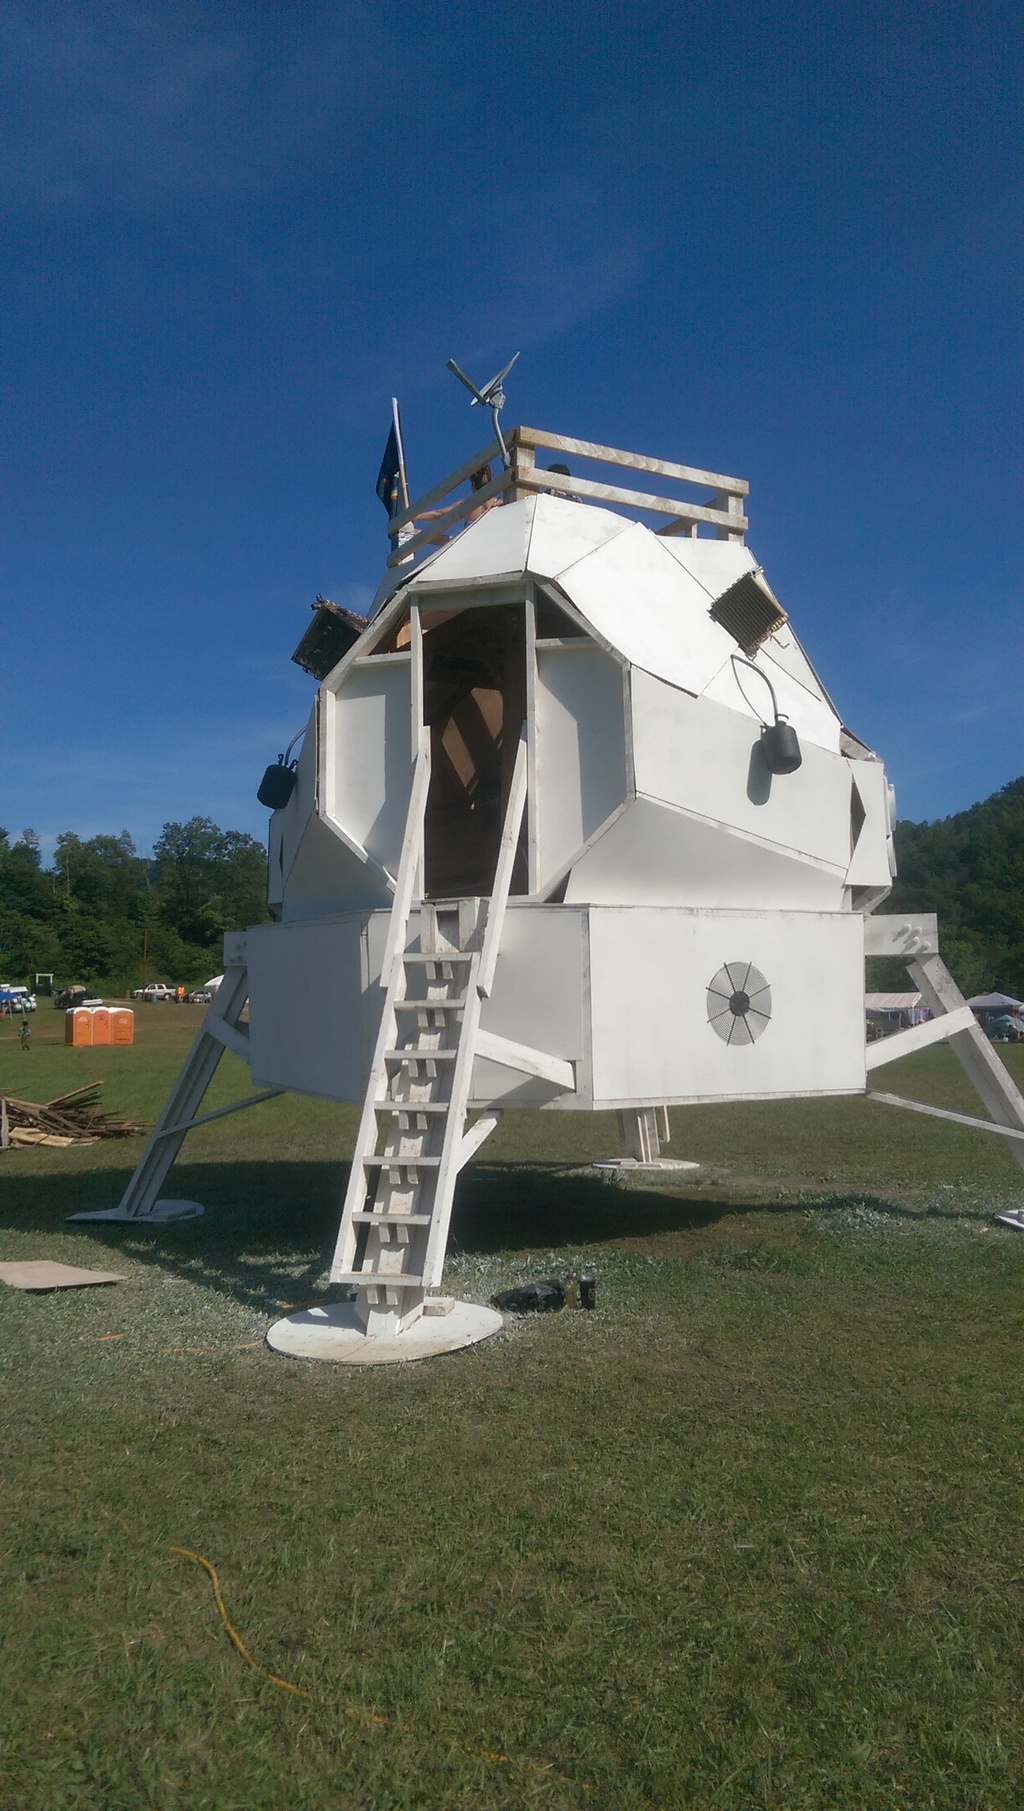
\includegraphics[width=\columnwidth]{images/2017Effigy_small.jpg}
\fi

% \vspace{3cm}
% 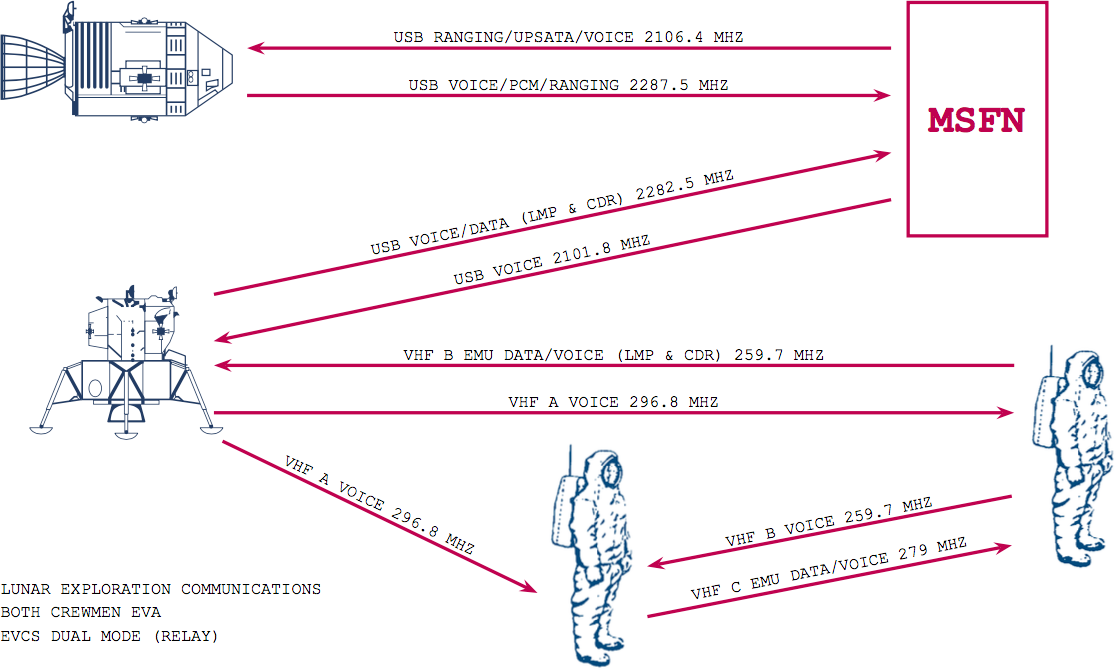
\includegraphics[width=\textwidth]{images/communication1.png}

% \subsection{No Car Camping}
% After checking in at the Greeter Station, you will be directed to unload your gear and then park your vehicle in the designated parking area, away from camping and event areas.  
% Only registered Art Cars, hybrid vehicles registered as generators (must be disguised and pimped out) or those needed by handicapped participants can stay with you at your campsite (must be covered up and decorated as well. They can't be driven during the event (with the exception of registered art cars)

% \subsection{Pets / Service Animals}
% \todo[inline]{BOD: please check; this is an abbreviated version that is more clear (to Raptor)}
% \begin{itemize}
% \item NO PETS ARE ALLOWED AT THIS EVENT
% \item Only working service animals are allowed on The Moon. Service animals are defined as dogs (or certain miniature horses) that are
%   \begin{itemize}
%   \item individually trained
%   \item identified as such to do work or perform tasks for people with disabilities.
%   \item Service animals must remain LEASHED and under control at ALL TIMES and will be asked to leave if the animal’s handler does not take effective action to control it.
%   \end{itemize}
% \item If you require a service animal to fully access the event, please inform us by no later than May 14, 2018 so that we can work with you to ensure comfort level for you and your service dog.
% \item No other animals may be brought or kept on the event premises. This includes
%   \begin{itemize}
%   \item Therapy animals
%   \item Emotional support animals
%   \item Personal pets
%   \end{itemize}
% \end{itemize}


